\documentclass{article}
\usepackage{graphicx}
\usepackage{fancyhdr}
\pagestyle{fancy}
\lhead{Ruicheng Wu}
\rhead{07/19/2017}
\chead{Homework 9}

\begin{document}
1.

a)
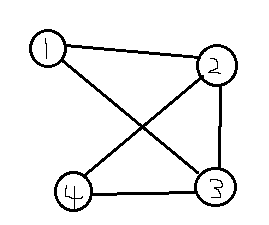
\includegraphics[scale=.5]{HW9_a.png}

b)
D(G)=\[
\left[ \begin {array}{ccccc}
2000\\
0300\\
0030\\
0002\\
\end{array} \right]
\]

L(G)=A(G)-D(G)=\[
\left[ \begin {array}{ccccc}
2&{-1}&{-1}&0\\
{-1}&3&{-1}&{-1}\\
{-1}&{-1}&3&{-1}\\
0&{-1}&{-1}&2\\
\end{array} \right]
\]

c)
According to (Kirchoff ’s Matrix Tree Theorem),number of labeled spanning trees of G is det L':

\[det
\left[ \begin {array}{ccccc}
3&{-1}&{-1}\\
{-1}&3&{-1}\\
{-1}&{-1}&2\\
\end{array} \right]
=8\]

So there are 8 labelled different spanning tree.

2.

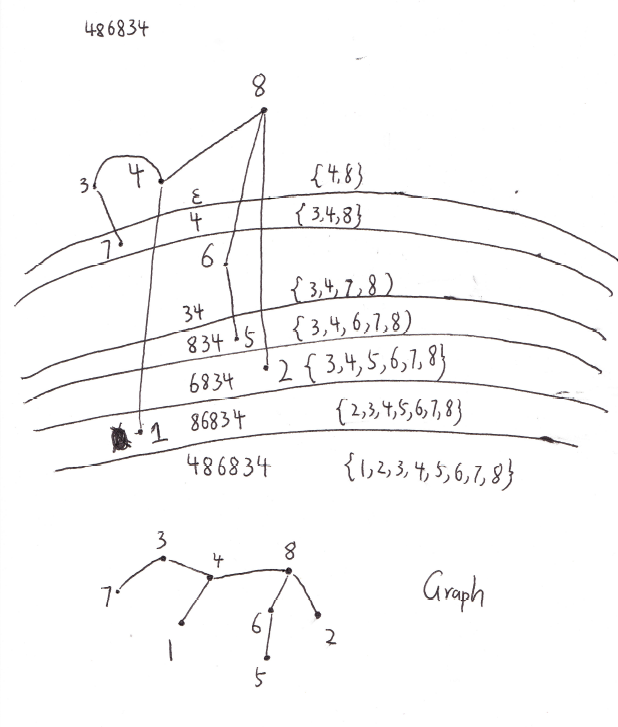
\includegraphics[scale=.9]{HW9_2.png}

3.

Draw all these trees:

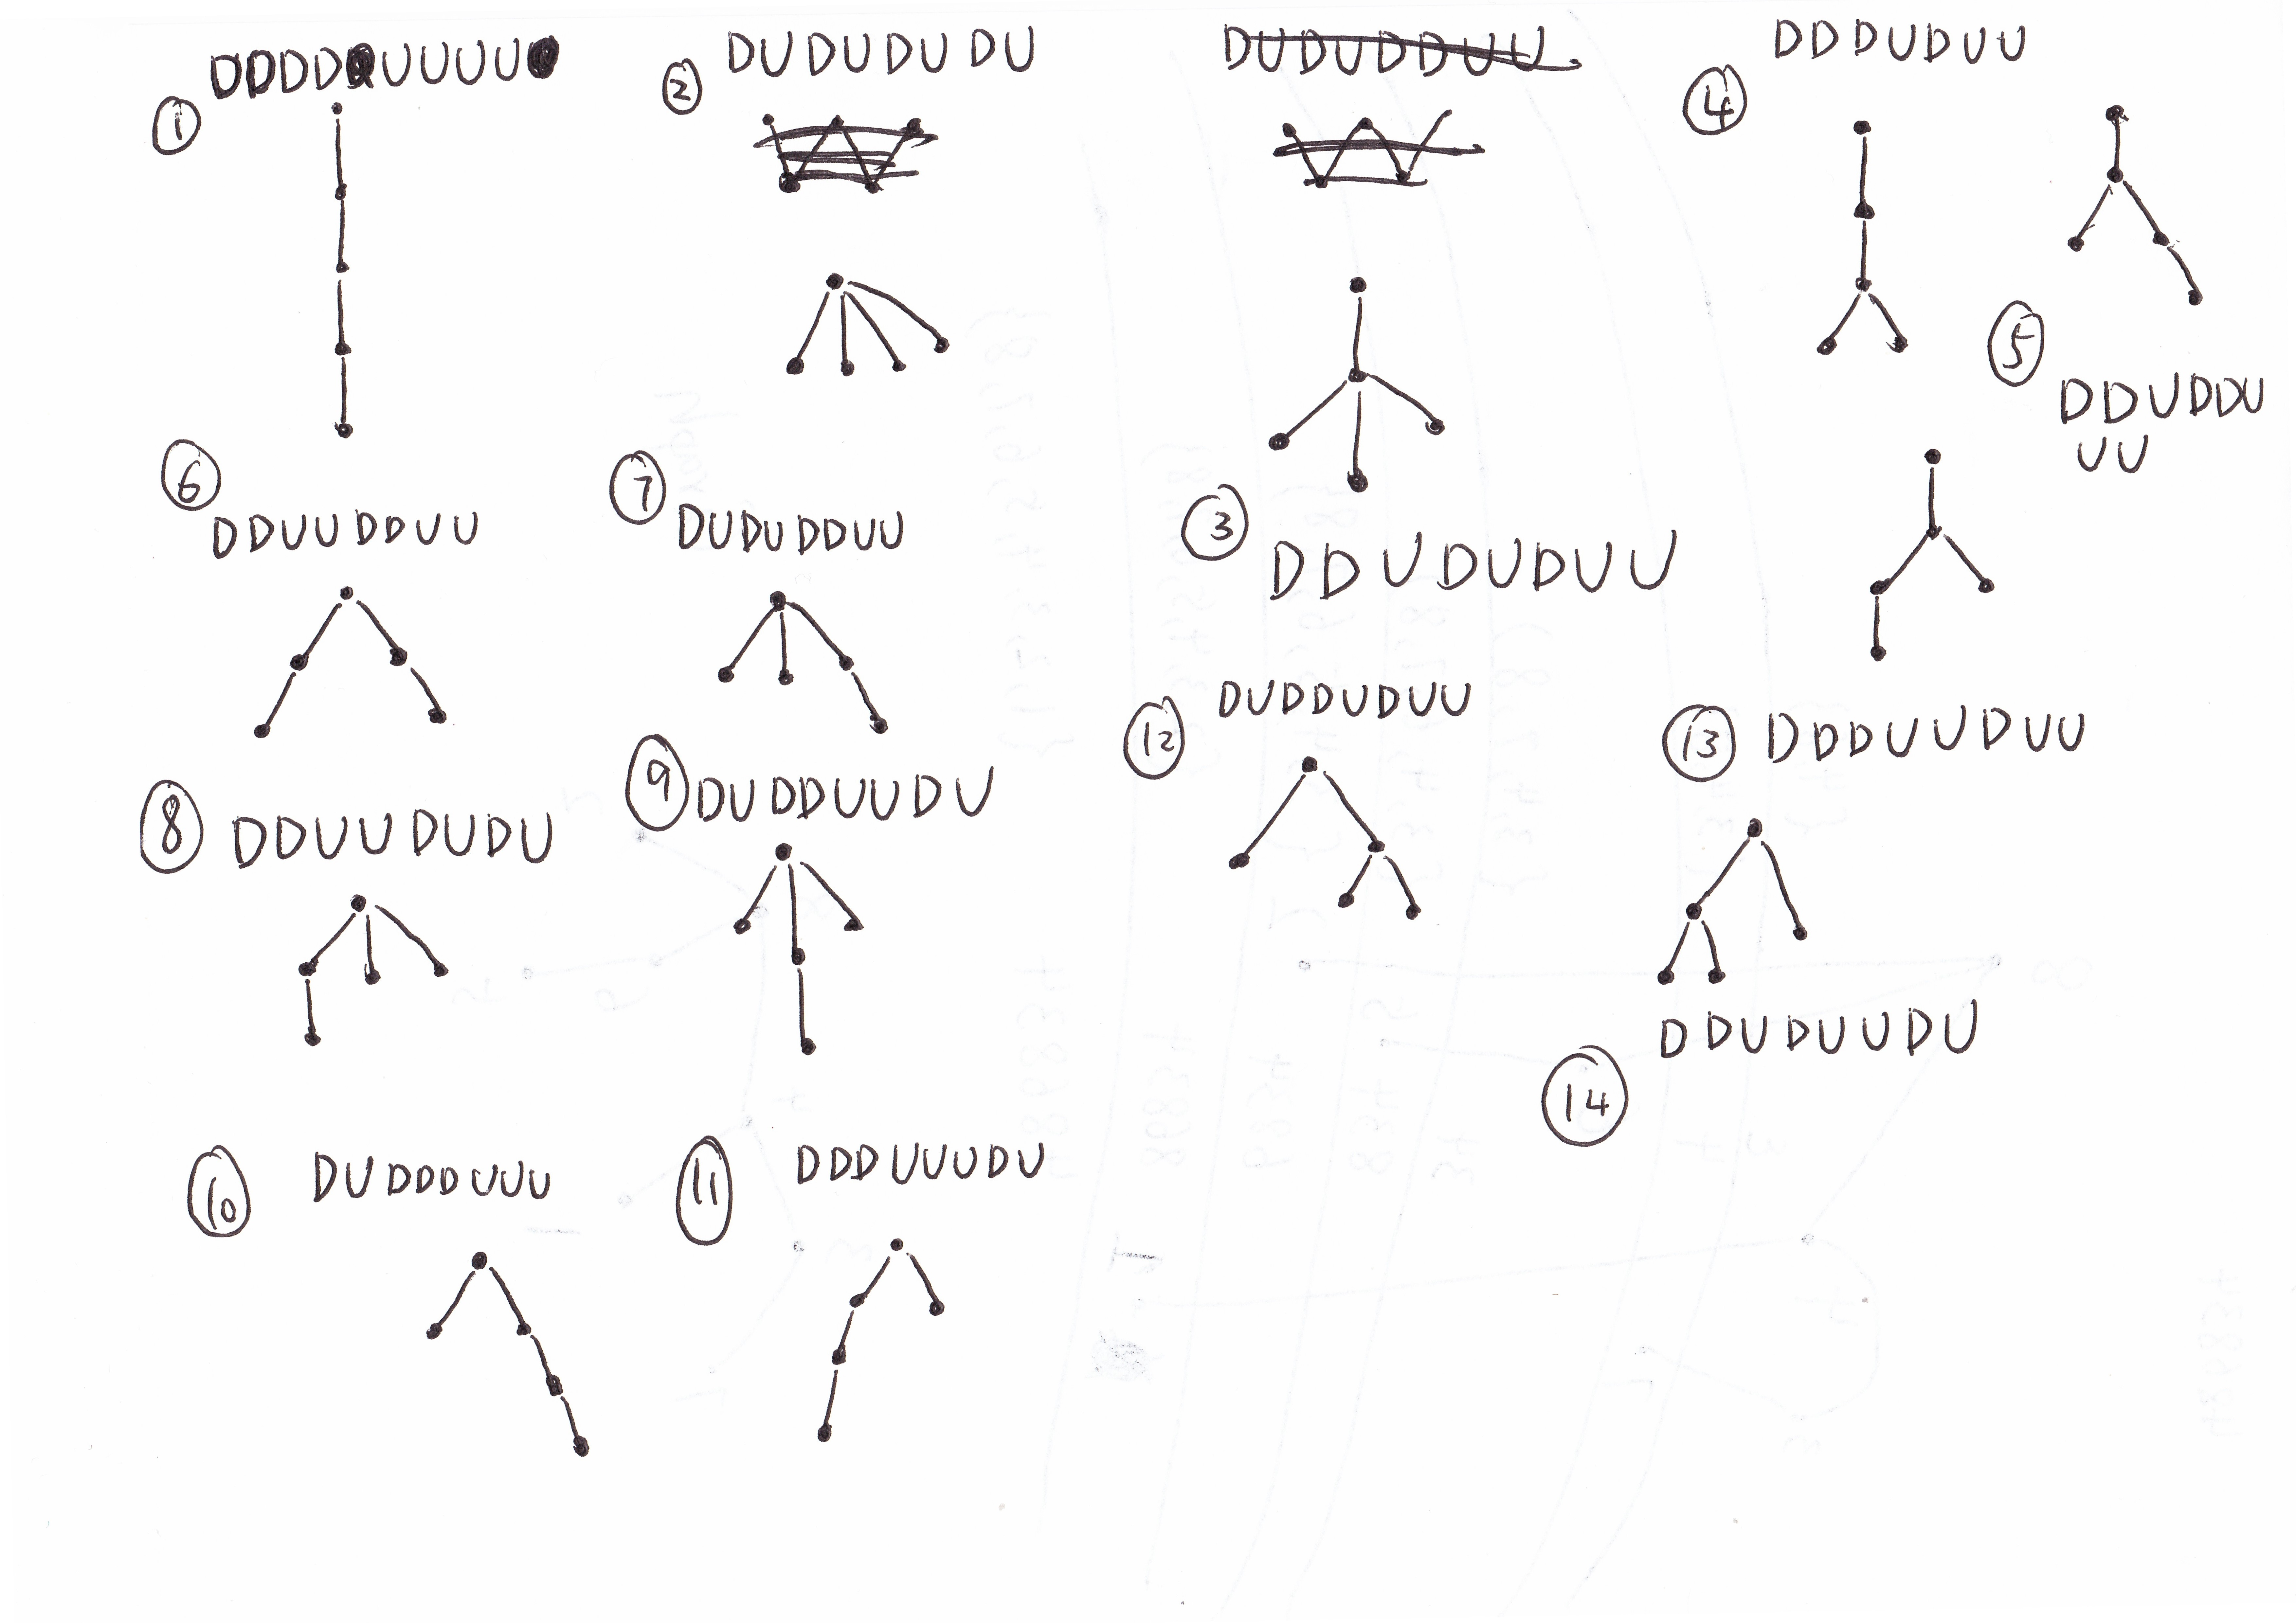
\includegraphics[scale=.5]{HW9_3.jpg}

According to formula:

$$C(n) = \frac{1}{n+1}*C(2n,n)= \frac{1}{5}*C(8,4) = 14$$

and we know that each traversal is unique for one tree. So this means we have successfully draw all 4-edges tree.








\end{document}